\documentclass[]{book}
\usepackage{lmodern}
\usepackage{amssymb,amsmath}
\usepackage{ifxetex,ifluatex}
\usepackage{fixltx2e} % provides \textsubscript
\ifnum 0\ifxetex 1\fi\ifluatex 1\fi=0 % if pdftex
  \usepackage[T1]{fontenc}
  \usepackage[utf8]{inputenc}
\else % if luatex or xelatex
  \ifxetex
    \usepackage{mathspec}
  \else
    \usepackage{fontspec}
  \fi
  \defaultfontfeatures{Ligatures=TeX,Scale=MatchLowercase}
\fi
% use upquote if available, for straight quotes in verbatim environments
\IfFileExists{upquote.sty}{\usepackage{upquote}}{}
% use microtype if available
\IfFileExists{microtype.sty}{%
\usepackage{microtype}
\UseMicrotypeSet[protrusion]{basicmath} % disable protrusion for tt fonts
}{}
\usepackage{hyperref}
\hypersetup{unicode=true,
            pdftitle={Apostila do Minicurso: introdução ao pacote dplyr},
            pdfauthor={Msc.Elisângela C. Biazatti Douglas Vinícius Jossivana Macedo},
            pdfborder={0 0 0},
            breaklinks=true}
\urlstyle{same}  % don't use monospace font for urls
\usepackage{natbib}
\bibliographystyle{apalike}
\usepackage{color}
\usepackage{fancyvrb}
\newcommand{\VerbBar}{|}
\newcommand{\VERB}{\Verb[commandchars=\\\{\}]}
\DefineVerbatimEnvironment{Highlighting}{Verbatim}{commandchars=\\\{\}}
% Add ',fontsize=\small' for more characters per line
\usepackage{framed}
\definecolor{shadecolor}{RGB}{248,248,248}
\newenvironment{Shaded}{\begin{snugshade}}{\end{snugshade}}
\newcommand{\AlertTok}[1]{\textcolor[rgb]{0.94,0.16,0.16}{#1}}
\newcommand{\AnnotationTok}[1]{\textcolor[rgb]{0.56,0.35,0.01}{\textbf{\textit{#1}}}}
\newcommand{\AttributeTok}[1]{\textcolor[rgb]{0.77,0.63,0.00}{#1}}
\newcommand{\BaseNTok}[1]{\textcolor[rgb]{0.00,0.00,0.81}{#1}}
\newcommand{\BuiltInTok}[1]{#1}
\newcommand{\CharTok}[1]{\textcolor[rgb]{0.31,0.60,0.02}{#1}}
\newcommand{\CommentTok}[1]{\textcolor[rgb]{0.56,0.35,0.01}{\textit{#1}}}
\newcommand{\CommentVarTok}[1]{\textcolor[rgb]{0.56,0.35,0.01}{\textbf{\textit{#1}}}}
\newcommand{\ConstantTok}[1]{\textcolor[rgb]{0.00,0.00,0.00}{#1}}
\newcommand{\ControlFlowTok}[1]{\textcolor[rgb]{0.13,0.29,0.53}{\textbf{#1}}}
\newcommand{\DataTypeTok}[1]{\textcolor[rgb]{0.13,0.29,0.53}{#1}}
\newcommand{\DecValTok}[1]{\textcolor[rgb]{0.00,0.00,0.81}{#1}}
\newcommand{\DocumentationTok}[1]{\textcolor[rgb]{0.56,0.35,0.01}{\textbf{\textit{#1}}}}
\newcommand{\ErrorTok}[1]{\textcolor[rgb]{0.64,0.00,0.00}{\textbf{#1}}}
\newcommand{\ExtensionTok}[1]{#1}
\newcommand{\FloatTok}[1]{\textcolor[rgb]{0.00,0.00,0.81}{#1}}
\newcommand{\FunctionTok}[1]{\textcolor[rgb]{0.00,0.00,0.00}{#1}}
\newcommand{\ImportTok}[1]{#1}
\newcommand{\InformationTok}[1]{\textcolor[rgb]{0.56,0.35,0.01}{\textbf{\textit{#1}}}}
\newcommand{\KeywordTok}[1]{\textcolor[rgb]{0.13,0.29,0.53}{\textbf{#1}}}
\newcommand{\NormalTok}[1]{#1}
\newcommand{\OperatorTok}[1]{\textcolor[rgb]{0.81,0.36,0.00}{\textbf{#1}}}
\newcommand{\OtherTok}[1]{\textcolor[rgb]{0.56,0.35,0.01}{#1}}
\newcommand{\PreprocessorTok}[1]{\textcolor[rgb]{0.56,0.35,0.01}{\textit{#1}}}
\newcommand{\RegionMarkerTok}[1]{#1}
\newcommand{\SpecialCharTok}[1]{\textcolor[rgb]{0.00,0.00,0.00}{#1}}
\newcommand{\SpecialStringTok}[1]{\textcolor[rgb]{0.31,0.60,0.02}{#1}}
\newcommand{\StringTok}[1]{\textcolor[rgb]{0.31,0.60,0.02}{#1}}
\newcommand{\VariableTok}[1]{\textcolor[rgb]{0.00,0.00,0.00}{#1}}
\newcommand{\VerbatimStringTok}[1]{\textcolor[rgb]{0.31,0.60,0.02}{#1}}
\newcommand{\WarningTok}[1]{\textcolor[rgb]{0.56,0.35,0.01}{\textbf{\textit{#1}}}}
\usepackage{longtable,booktabs}
\usepackage{graphicx,grffile}
\makeatletter
\def\maxwidth{\ifdim\Gin@nat@width>\linewidth\linewidth\else\Gin@nat@width\fi}
\def\maxheight{\ifdim\Gin@nat@height>\textheight\textheight\else\Gin@nat@height\fi}
\makeatother
% Scale images if necessary, so that they will not overflow the page
% margins by default, and it is still possible to overwrite the defaults
% using explicit options in \includegraphics[width, height, ...]{}
\setkeys{Gin}{width=\maxwidth,height=\maxheight,keepaspectratio}
\IfFileExists{parskip.sty}{%
\usepackage{parskip}
}{% else
\setlength{\parindent}{0pt}
\setlength{\parskip}{6pt plus 2pt minus 1pt}
}
\setlength{\emergencystretch}{3em}  % prevent overfull lines
\providecommand{\tightlist}{%
  \setlength{\itemsep}{0pt}\setlength{\parskip}{0pt}}
\setcounter{secnumdepth}{5}
% Redefines (sub)paragraphs to behave more like sections
\ifx\paragraph\undefined\else
\let\oldparagraph\paragraph
\renewcommand{\paragraph}[1]{\oldparagraph{#1}\mbox{}}
\fi
\ifx\subparagraph\undefined\else
\let\oldsubparagraph\subparagraph
\renewcommand{\subparagraph}[1]{\oldsubparagraph{#1}\mbox{}}
\fi

%%% Use protect on footnotes to avoid problems with footnotes in titles
\let\rmarkdownfootnote\footnote%
\def\footnote{\protect\rmarkdownfootnote}

%%% Change title format to be more compact
\usepackage{titling}

% Create subtitle command for use in maketitle
\providecommand{\subtitle}[1]{
  \posttitle{
    \begin{center}\large#1\end{center}
    }
}

\setlength{\droptitle}{-2em}

  \title{Apostila do Minicurso: introdução ao pacote dplyr}
    \pretitle{\vspace{\droptitle}\centering\huge}
  \posttitle{\par}
    \author{Msc.Elisângela C. BiazattiDouglas ViníciusJossivana Macedo}
    \preauthor{\centering\large\emph}
  \postauthor{\par}
      \predate{\centering\large\emph}
  \postdate{\par}
    \date{22 de outubro de 2019}

\usepackage{booktabs}

\begin{document}
\maketitle

{
\setcounter{tocdepth}{1}
\tableofcontents
}
\hypertarget{prefuxe1cio}{%
\chapter{Prefácio}\label{prefuxe1cio}}

Este material foi elaborado com o proprósito de um minicurso, que tem como objetivo apresentar algumas ideias das funções básicas do pacote \texttt{dplyr}, podemos usar um computador e um pouco de criatividade para explorar essas idéias em uma variedade de situações. Usamos R com o RStudio para fazer todo o nosso trabalho.

O livro \href{https://r4ds.had.co.nz/}{R for data science} é o mais indicado para aprender sobre o universo \texttt{tidyverse}. Nesse minicurso abordamos mais sobre a gramática das funções básicas do \texttt{dplyr} alguns exemplos e exercícios abordados.

\hypertarget{puxfablico-alvo}{%
\section{Público-alvo}\label{puxfablico-alvo}}

\begin{itemize}
\tightlist
\item
  Estudantes de estatística que desejam ganhar tempo nos trabalhos da faculdade;
\item
  Acadêmicos com interesse em tornar suas análises e códigos mais legíveis em R.
\end{itemize}

\hypertarget{conteuxfado}{%
\section{Conteúdo:}\label{conteuxfado}}

\begin{verbatim}
- Primeiro dia (22/10): R básico, swirl, organização de dados, exercícios; 
- Segundo dia (23/10): select(), filter(), arrange(), mutate(), summarise(), exercícios;
- Terceiro dia (24/10): agrupar dados, combinar conjuntos de dados.
\end{verbatim}

\hypertarget{pruxe9-requisitos}{%
\section{Pré-requisitos}\label{pruxe9-requisitos}}

\hypertarget{intro}{%
\chapter{Introdução}\label{intro}}

\begin{quote}
``Existem apenas dois tipos de idiomas: os que as pessoas reclamam e os que ninguém usa''. - Bjarne Stroustrup
\end{quote}

O modelo típico de análise de dados é similar:

\begin{center}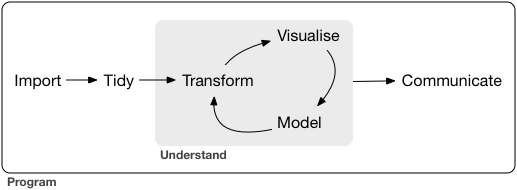
\includegraphics[width=0.75\linewidth]{imagens/data-science} \end{center}

Primeiramente, você deve \textbf{importar} seus dados para o R. Significa que você pega os dados armazenados em um arquivo, banco de dados ou API da Web e carrega-os em um data frames no R.

Logo após, a ideia é \textbf{organizá}-los. Significa armazená-los de forma consistente.

Depois de arrumar os dados, o próximo passo é \textbf{transformá}-los. Significa restringir observações de interesse, criar novas variáveis

Depois de organizar os dados com as variáveis necessárias, existem dois mecanismos principais de geração de conhecimento: visualização e modelagem. Eles têm pontos fortes e fracos complementares, portanto qualquer análise real se repetirá entre eles várias vezes.

A \textbf{visualização} é uma atividade fundamentalmente humana. Uma boa visualização mostrará coisas que você não esperava, ou fará novas perguntas sobre os dados.

\textbf{Modelos} são ferramentas complementares para visualização. Depois de fazer suas perguntas suficientemente precisas, você pode usar um modelo para respondê-las.

O último passo da ciência de dados é a \textbf{comunicação}, uma parte absolutamente crítica de qualquer projeto de análise de dados. Não importa o quão bem seus modelos e visualização levaram você a entender os dados, a menos que você também possa comunicar seus resultados a outras pessoas.

Ao redor de todas essas ferramentas está a programação. A programação é uma ferramenta transversal que você usa em todas as partes do projeto. Você não precisa ser um programador especialista para ser um cientista de dados, mas aprender mais sobre programação compensa, porque se tornar um programador melhor permite automatizar tarefas comuns e resolver novos problemas com maior facilidade.

\hypertarget{r-e-rstudio}{%
\section{R e RStudio}\label{r-e-rstudio}}

A primeira coisa que você precisa fazer para iniciar o R é instalá-lo no seu computador. O R funciona em praticamente todas as plataformas disponíveis, incluindo os sistemas Windows, Mac OS X e Linux amplamente disponíveis.

Uma nova versão principal do R sai uma vez por ano, e há 2 ou 3 versões menores a cada ano. É uma boa ideia atualizar regularmente. A atualização pode ser um pouco complicada, especialmente para as versões principais, que exigem a reinstalação de todos os seus pacotes.

Há também um ambiente de desenvolvimento integrado (IDE) disponível para o R, construído pelo RStudio. IDE, do inglês \textbf{Integrated Development Environment} ou Ambiente de Desenvolvimento Integrado, é um programa de computador que reúne características e ferramentas de apoio ao desenvolvimento de software com o objetivo de agilizar este processo. O RStudio é atualizado duas vezes por ano. Quando uma nova versão estiver disponível, o RStudio informará você.

Você pode ver como instalar o R e o RStudio aqui:

\begin{itemize}
\tightlist
\item
  \href{https://www.youtube.com/watch?v=orjLGFmx6l4}{Instalando o RStudio}
\end{itemize}

Após instalado, o R tem uma interface assim, com apenas o console para digitar comandos:

\begin{center}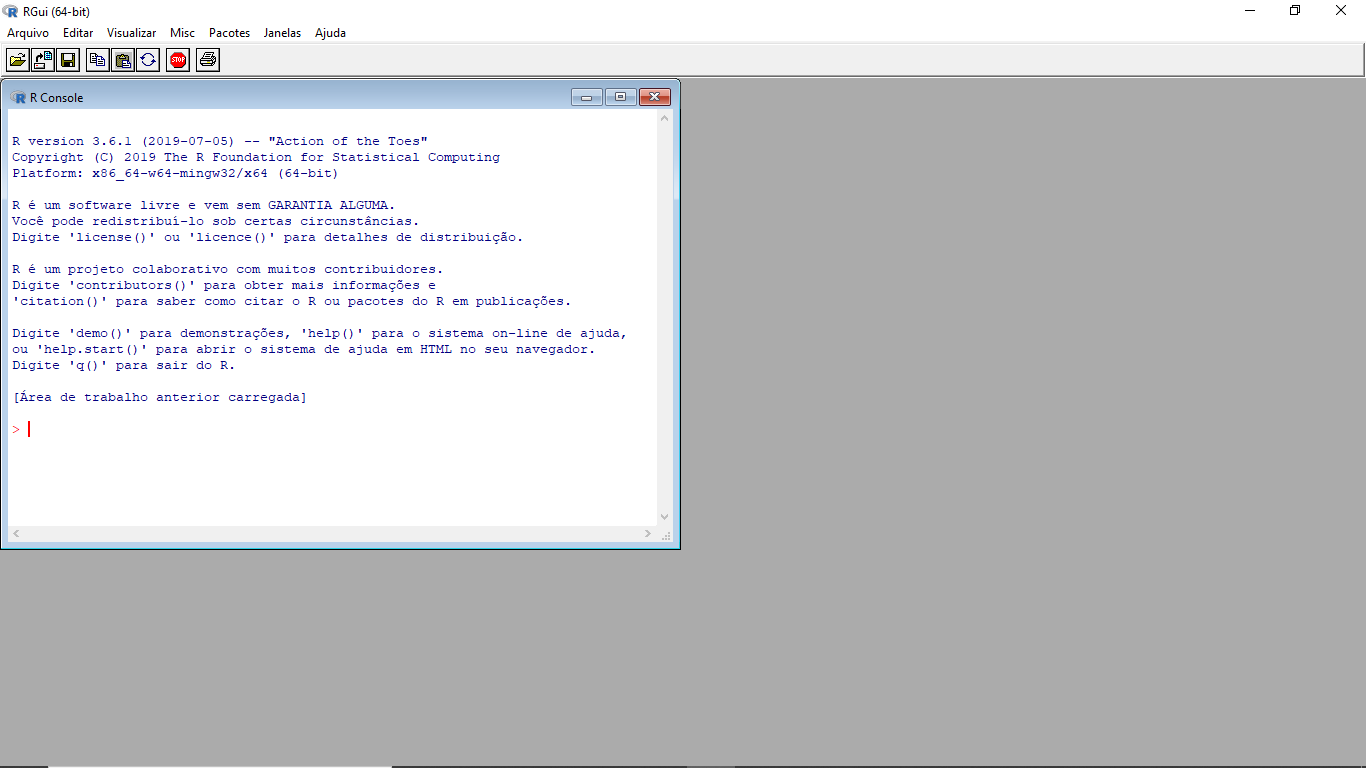
\includegraphics[width=0.9\linewidth]{imagens/r-project} \end{center}

Experimente um comando: 2+2, cujo output é 4:

\begin{Shaded}
\begin{Highlighting}[]
\DecValTok{2} \OperatorTok{+}\StringTok{ }\DecValTok{2}
\end{Highlighting}
\end{Shaded}

\begin{verbatim}
## [1] 4
\end{verbatim}

E a interface do RStudio é dividida, inicialmente, em 3 partes:

\begin{center}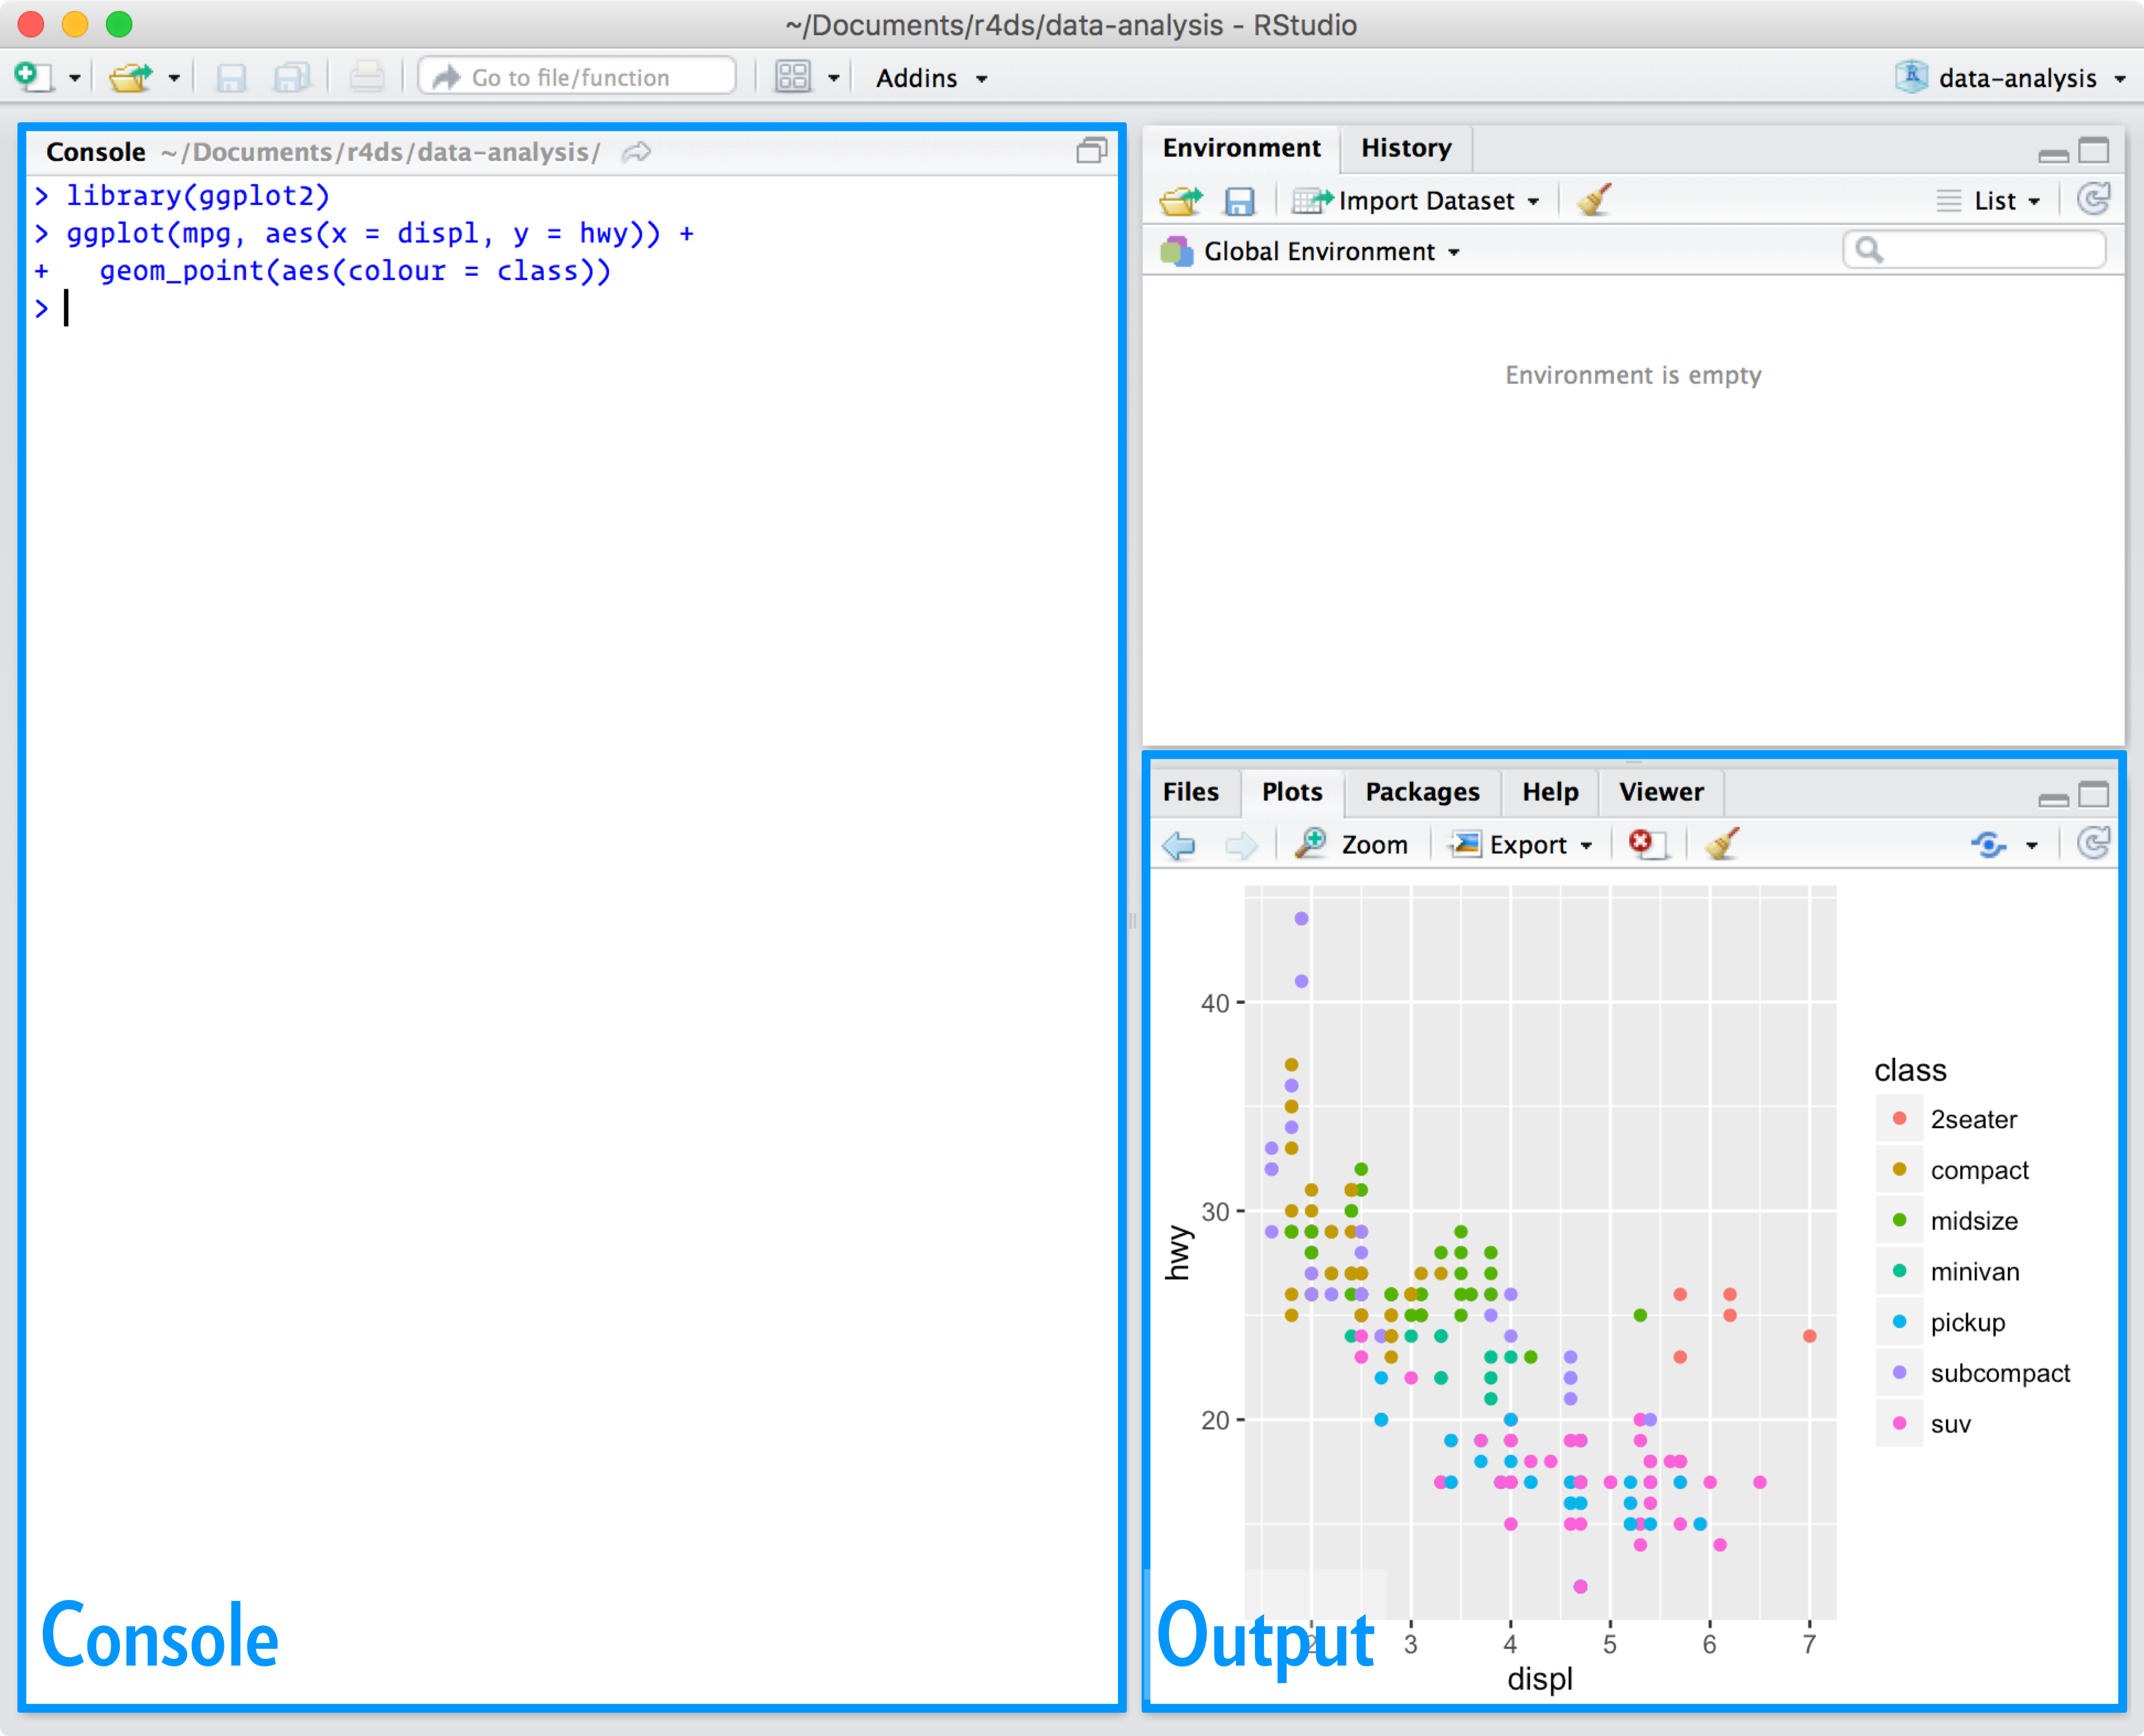
\includegraphics[width=0.9\linewidth]{imagens/rstudio-console} \end{center}

Do lado esquerdo fica o console, onde os comandos podem ser digitados e onde ficam os \emph{outputs}.

No lado superior direito há duas abas:

-i) \emph{Environment}, que é onde ficam armazendos os objetos criados, bases de dados importadas, etc; e

-ii) \emph{History}, onde ficam o histórico dos comandos executados.

A forma mais eficiente e prática de usar o R ou o RStudio é através de um \emph{script}. No RStudio, vá em \emph{File} → \emph{New File} → \emph{R Script}. A interface agora fica dividida em 4 partes:

\begin{center}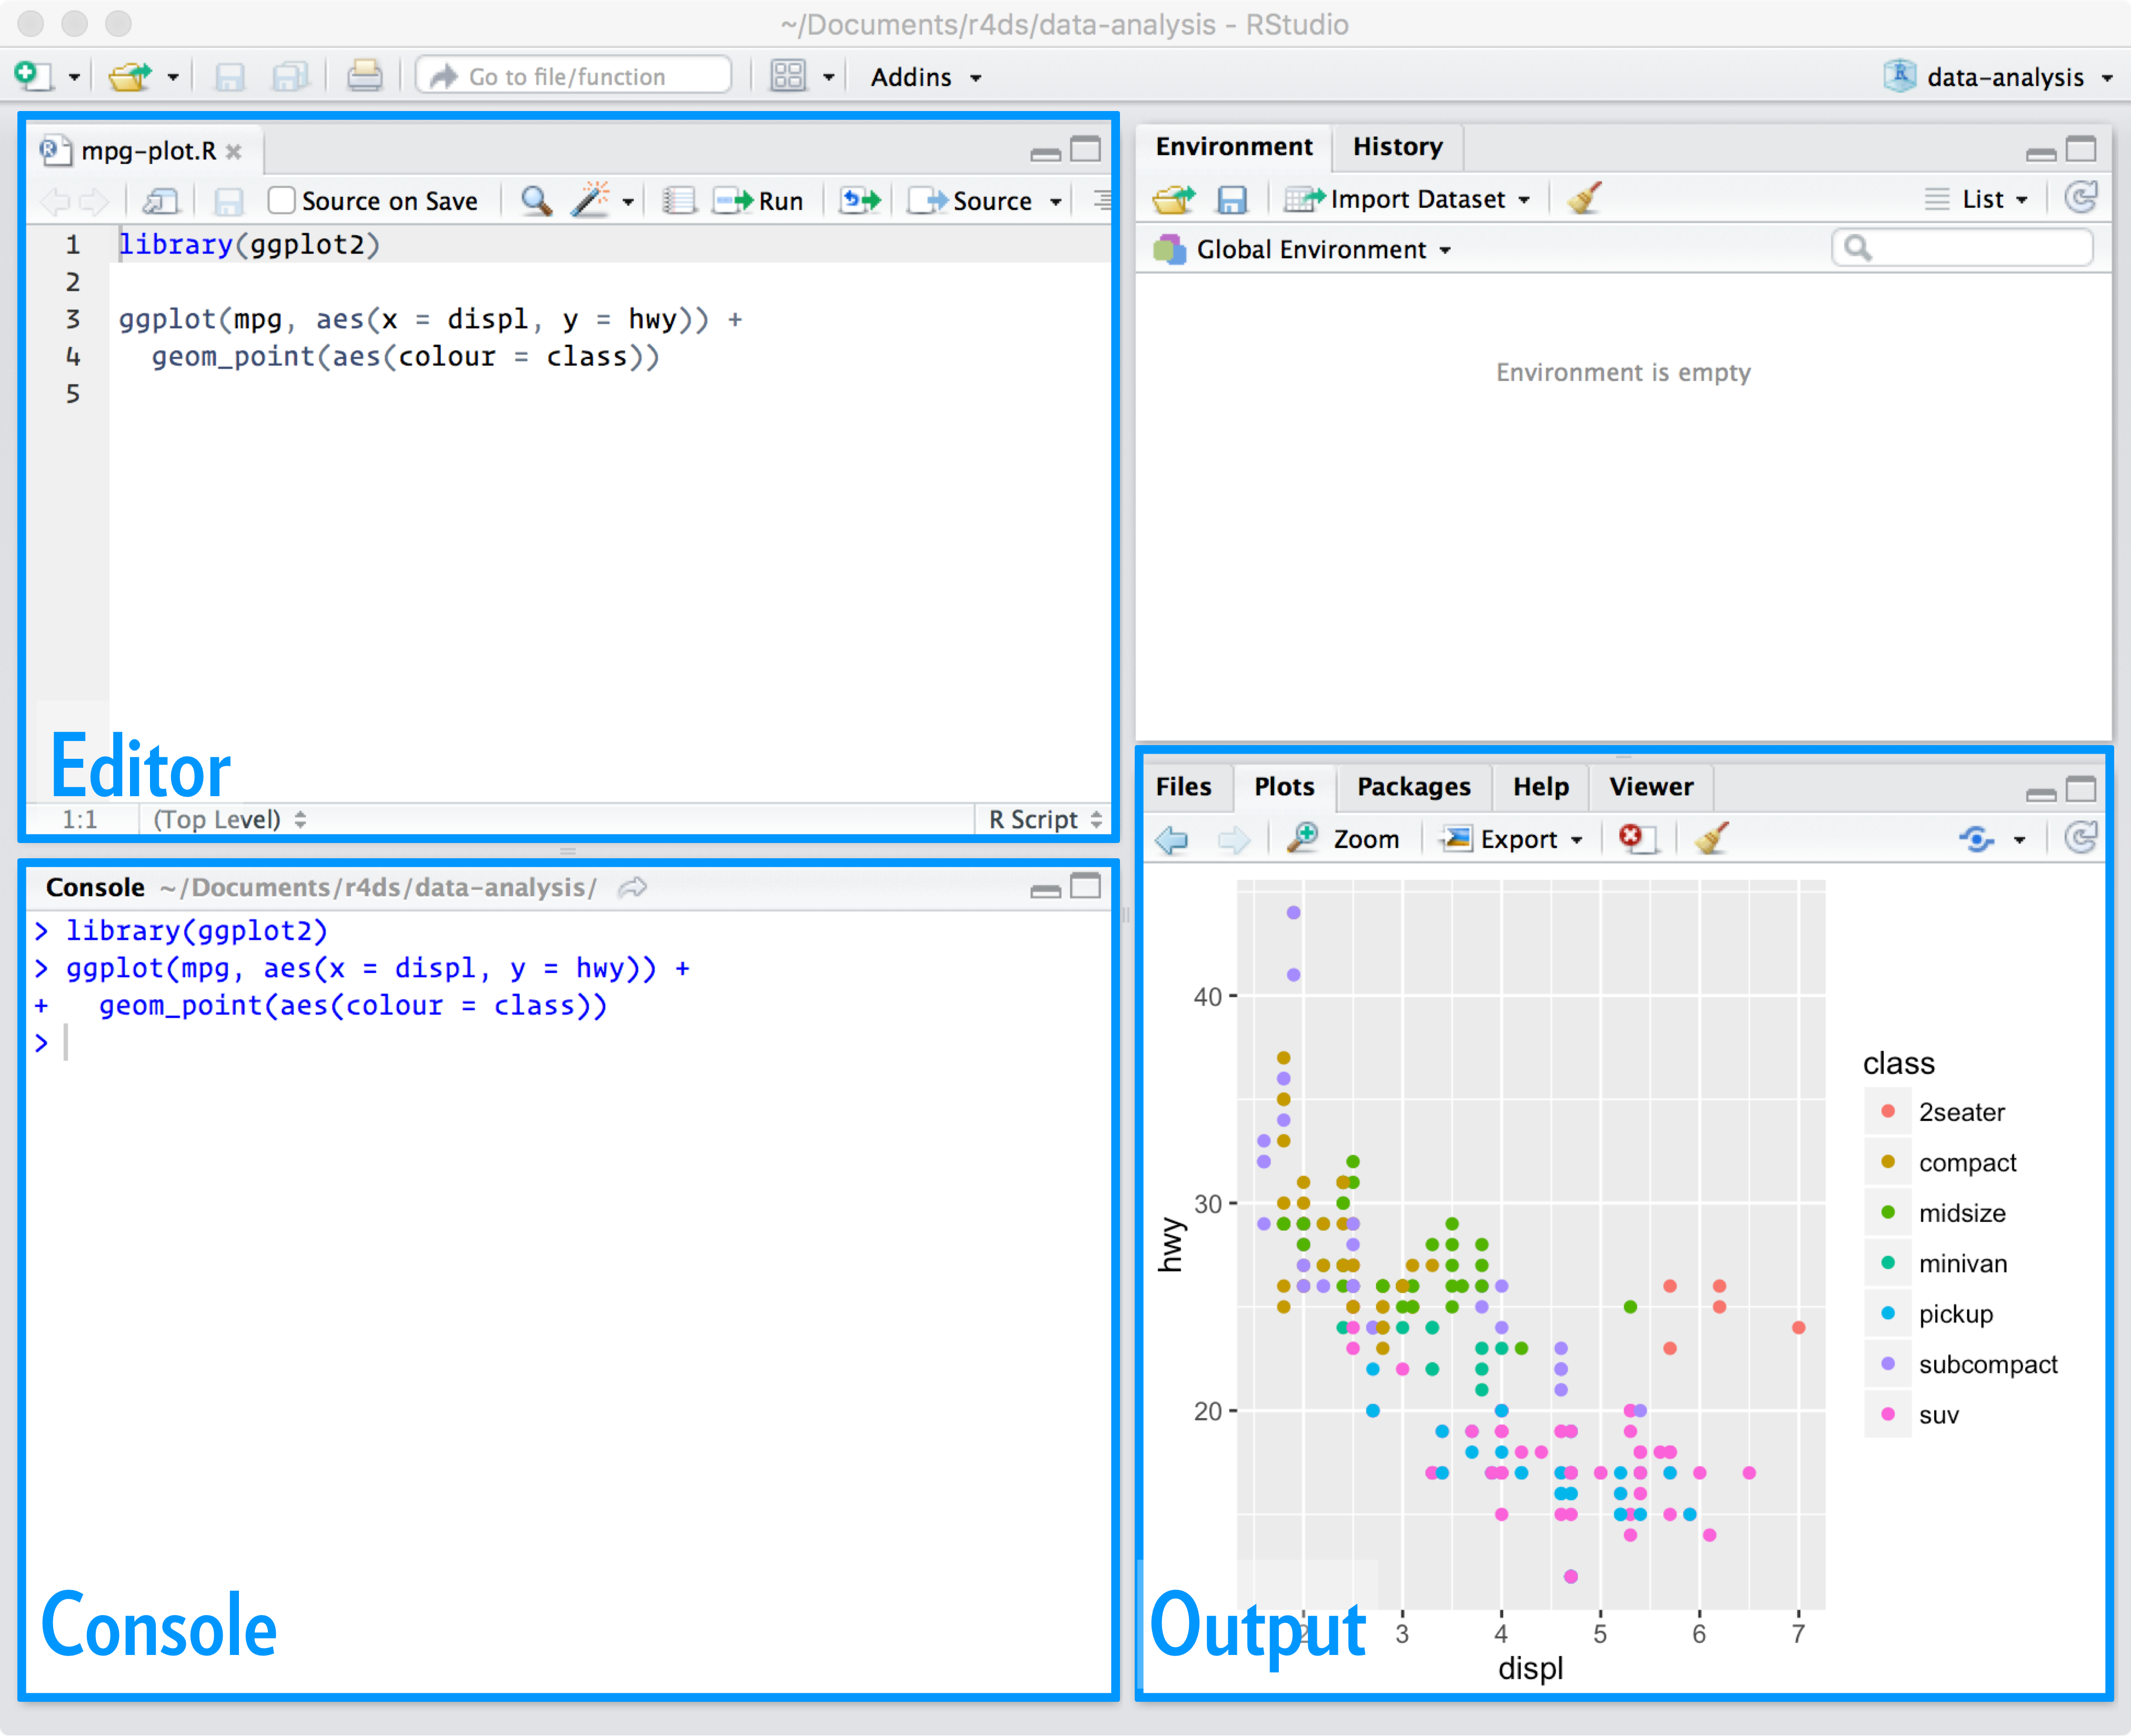
\includegraphics[width=0.9\linewidth]{imagens/rstudio-editor} \end{center}

No \emph{script} você pode digitar comandos a serem executados e também comentários.

\hypertarget{swirl}{%
\section{\texorpdfstring{\emph{swirl}}{swirl}}\label{swirl}}

O \emph{swirl} é um pacote do R construído para transformar o console em uma ferramenta interativa para aprender R. \emph{swirl} ensina programação de R e ciência de dados interativamente, no seu próprio ritmo e diretamente no console do R. Para entender melhor do projeto, veja \url{http://swirlstats.com/}. Em \url{http://swirlstats.com/students}. Nestes endereços de são dados os detalhes sobre como usar o \emph{swirl}. Uma vez intalado e carregado o pacote, você é levado a efetuar tarefas:

\begin{center}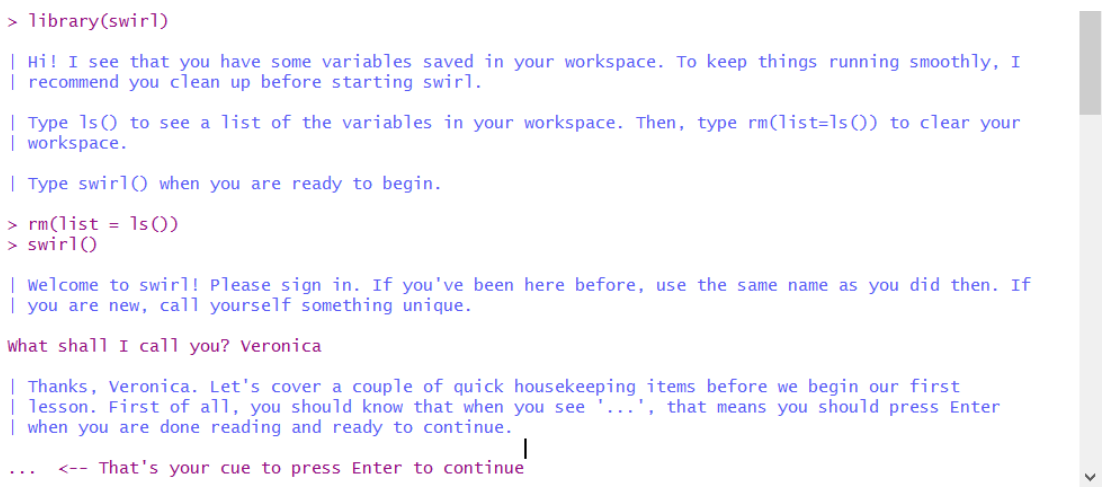
\includegraphics[width=0.9\linewidth]{imagens/swirl} \end{center}

O \emph{swirl} dá acesso às tarefas de cursos de R que estão disponíveis também no Coursera, como o \emph{R Programming}: \emph{The basics of programming in R}, em \url{https://pt.coursera.org/learn/r-programming}. Além deste, estão
disponíveis no \emph{swirl}: \emph{Regression Models: The basics of regression modeling in R, Statistical Inference: The basics of statistical inference in R, e Exploratory Data Analysis: The basics of exploring data in R}.

\hypertarget{universo-tidyverse}{%
\section{\texorpdfstring{Universo \texttt{tidyverse}}{Universo tidyverse}}\label{universo-tidyverse}}

\begin{center}
\includegraphics[width=0.25\linewidth]{imagens/hex-tidyverse} \end{center}

O tidyverse é uma coleção opinativa de pacotes R projetados para ciência de dados. Todos os pacotes compartilham uma filosofia de design, gramática e estruturas de dados subjacentes.

Os princípios fundamentais do \texttt{tidyverse} são:

\begin{itemize}
\tightlist
\item
  1.Reutilizar estruturas de dados existentes;
\item
  2.Organizar funções simples usando o pipe;
\item
  3.Aderir à programação funcional;
\item
  4.Projetado para ser usado por seres humanos.
\end{itemize}

Assim como o processo típico do passo a passo apresentando anteriormente para análise de dados, o \texttt{tidyverse} é a ferramenta que o ajuda eficientemente a executar este processo.

\begin{Shaded}
\begin{Highlighting}[]
\KeywordTok{library}\NormalTok{(tidyverse) }\CommentTok{#Carregar o pacote.}
\end{Highlighting}
\end{Shaded}

\begin{verbatim}
## -- Attaching packages ------------------------------ tidyverse 1.2.1 --
\end{verbatim}

\begin{verbatim}
## v ggplot2 3.2.1     v purrr   0.3.2
## v tibble  2.1.3     v dplyr   0.8.3
## v tidyr   1.0.0     v stringr 1.4.0
## v readr   1.3.1     v forcats 0.4.0
\end{verbatim}

\begin{verbatim}
## -- Conflicts --------------------------------- tidyverse_conflicts() --
## x dplyr::filter() masks stats::filter()
## x dplyr::lag()    masks stats::lag()
\end{verbatim}

\begin{Shaded}
\begin{Highlighting}[]
\KeywordTok{tidyverse_logo}\NormalTok{() }\CommentTok{#Logo}
\end{Highlighting}
\end{Shaded}

\begin{verbatim}
## * __  _    __   .    o           *  . 
##  / /_(_)__/ /_ ___  _____ _______ ___ 
## / __/ / _  / // / |/ / -_) __(_-</ -_)
## \__/_/\_,_/\_, /|___/\__/_/ /___/\__/ 
##      *  . /___/      o      .       *
\end{verbatim}

\hypertarget{o-que-uxe9-dados-organizados}{%
\chapter{O que é Dados organizados?}\label{o-que-uxe9-dados-organizados}}

\begin{quote}
``Famílias felizes são todas iguais; toda família infeliz é infeliz à sua maneira.'' -- Leo Tolstoi
\end{quote}

\begin{quote}
``Os conjuntos de dados organizados são todos iguais, mas todos os conjuntos de dados confusos são confusos à sua maneira.'' -- Hadley Wickham
\end{quote}

Você vai precisar instalar os pacotes \texttt{tidyr}, \texttt{devtools} e \texttt{DSR}. Para instalar tidyr e devtools, abra o RStudio e execute o comando:

\begin{Shaded}
\begin{Highlighting}[]
\KeywordTok{install.packages}\NormalTok{(}\KeywordTok{c}\NormalTok{(}\StringTok{"tidyr"}\NormalTok{, }\StringTok{"devtools"}\NormalTok{))}
\end{Highlighting}
\end{Shaded}

\texttt{DSR} é uma coleção de conjuntos de dados. Para instalar DSR, execute o comando:

\begin{Shaded}
\begin{Highlighting}[]
\NormalTok{devtools}\OperatorTok{::}\KeywordTok{install_github}\NormalTok{(}\StringTok{"garrettgman/DSR"}\NormalTok{)}
\end{Highlighting}
\end{Shaded}

Os dados tabulares podem ser organizados de várias maneiras. Os conjuntos de dados abaixo mostram os mesmos dados organizados de quatro maneiras diferentes, sendo que possuem as mesmas variáveis: país, ano, população e casos. Mas cada conjunto organiza os valores em forma de layout diferente.

\begin{Shaded}
\begin{Highlighting}[]
\KeywordTok{library}\NormalTok{(DSR)}
\end{Highlighting}
\end{Shaded}

\begin{verbatim}
## 
## Attaching package: 'DSR'
\end{verbatim}

\begin{verbatim}
## The following objects are masked from 'package:tidyr':
## 
##     population, table1, table2, table3, table5, who
\end{verbatim}

\begin{Shaded}
\begin{Highlighting}[]
\CommentTok{# Primeiro conjunto de dados.}
\NormalTok{table1}
\end{Highlighting}
\end{Shaded}

\begin{verbatim}
## # A tibble: 6 x 4
##   country      year  cases population
##   <fct>       <int>  <int>      <int>
## 1 Afghanistan  1999    745   19987071
## 2 Afghanistan  2000   2666   20595360
## 3 Brazil       1999  37737  172006362
## 4 Brazil       2000  80488  174504898
## 5 China        1999 212258 1272915272
## 6 China        2000 213766 1280428583
\end{verbatim}

\begin{Shaded}
\begin{Highlighting}[]
\CommentTok{# Segundo conjunto de dados.}
\NormalTok{table2}
\end{Highlighting}
\end{Shaded}

\begin{verbatim}
## # A tibble: 12 x 4
##    country      year key             value
##    <fct>       <int> <fct>           <int>
##  1 Afghanistan  1999 cases             745
##  2 Afghanistan  1999 population   19987071
##  3 Afghanistan  2000 cases            2666
##  4 Afghanistan  2000 population   20595360
##  5 Brazil       1999 cases           37737
##  6 Brazil       1999 population  172006362
##  7 Brazil       2000 cases           80488
##  8 Brazil       2000 population  174504898
##  9 China        1999 cases          212258
## 10 China        1999 population 1272915272
## 11 China        2000 cases          213766
## 12 China        2000 population 1280428583
\end{verbatim}

\begin{Shaded}
\begin{Highlighting}[]
\CommentTok{# Terceiro conjunto de dados.}
\NormalTok{table3}
\end{Highlighting}
\end{Shaded}

\begin{verbatim}
## # A tibble: 6 x 3
##   country      year rate             
##   <fct>       <int> <chr>            
## 1 Afghanistan  1999 745/19987071     
## 2 Afghanistan  2000 2666/20595360    
## 3 Brazil       1999 37737/172006362  
## 4 Brazil       2000 80488/174504898  
## 5 China        1999 212258/1272915272
## 6 China        2000 213766/1280428583
\end{verbatim}

O último conjunto de dados é uma coleção de duas tabelas.

\begin{Shaded}
\begin{Highlighting}[]
\CommentTok{# Quarto conjunto de dados.}
\NormalTok{table4 }\CommentTok{# cases}
\end{Highlighting}
\end{Shaded}

\begin{verbatim}
## # A tibble: 3 x 3
##   country     `1999` `2000`
##   <fct>        <int>  <int>
## 1 Afghanistan    745   2666
## 2 Brazil       37737  80488
## 3 China       212258 213766
\end{verbatim}

\begin{Shaded}
\begin{Highlighting}[]
\NormalTok{table5 }\CommentTok{# population}
\end{Highlighting}
\end{Shaded}

\begin{verbatim}
## # A tibble: 3 x 3
##   country         `1999`     `2000`
##   <fct>            <int>      <int>
## 1 Afghanistan   19987071   20595360
## 2 Brazil       172006362  174504898
## 3 China       1272915272 1280428583
\end{verbatim}

R segue um conjunto de convenções que tornam um layout de dados tabulares muito mais fácil de trabalhar do que outros. Seus dados serão mais fáceis de trabalhar no R se seguirem três regras:

\begin{itemize}
\tightlist
\item
  1.Cada variável no conjunto de dados é colocada em sua própria coluna;
\item
  2.Cada observação é colocada em sua própria linha;
\item
  3.Cada valor é colocado em sua própria célula.
\end{itemize}

Os dados que satisfazem essas regras são conhecidos como dados organizados. Observe que \texttt{table1} são dados organizados.

\begin{center}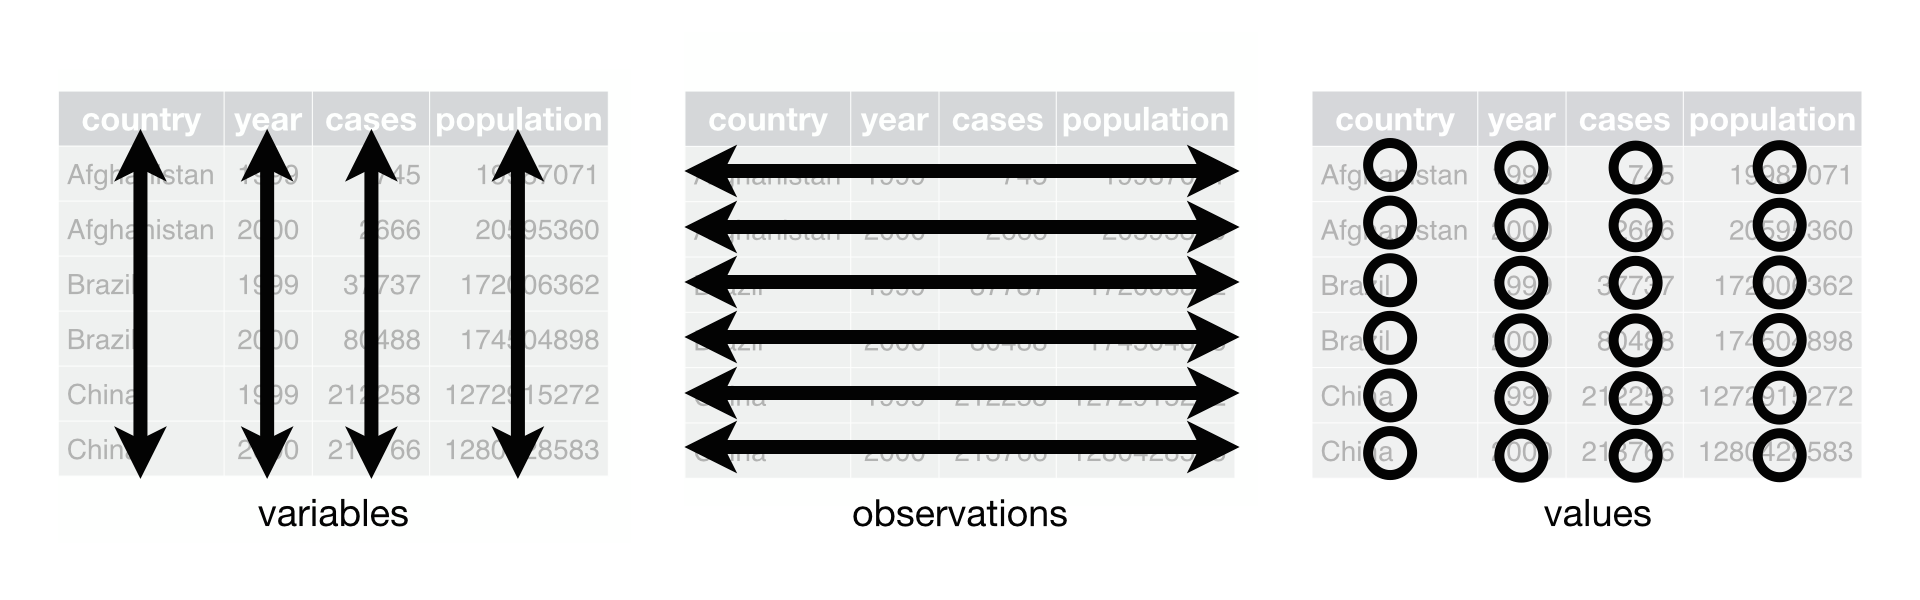
\includegraphics[width=0.9\linewidth]{imagens/tidy-1} \end{center}

Em \texttt{table1}, cada variável é colocada em sua própria coluna, cada observação em sua própria linha e cada valor em sua própria célula.

\hypertarget{introduuxe7uxe3o-ao-tidyr}{%
\section{\texorpdfstring{Introdução ao \texttt{tidyr}}{Introdução ao tidyr}}\label{introduuxe7uxe3o-ao-tidyr}}

\begin{center}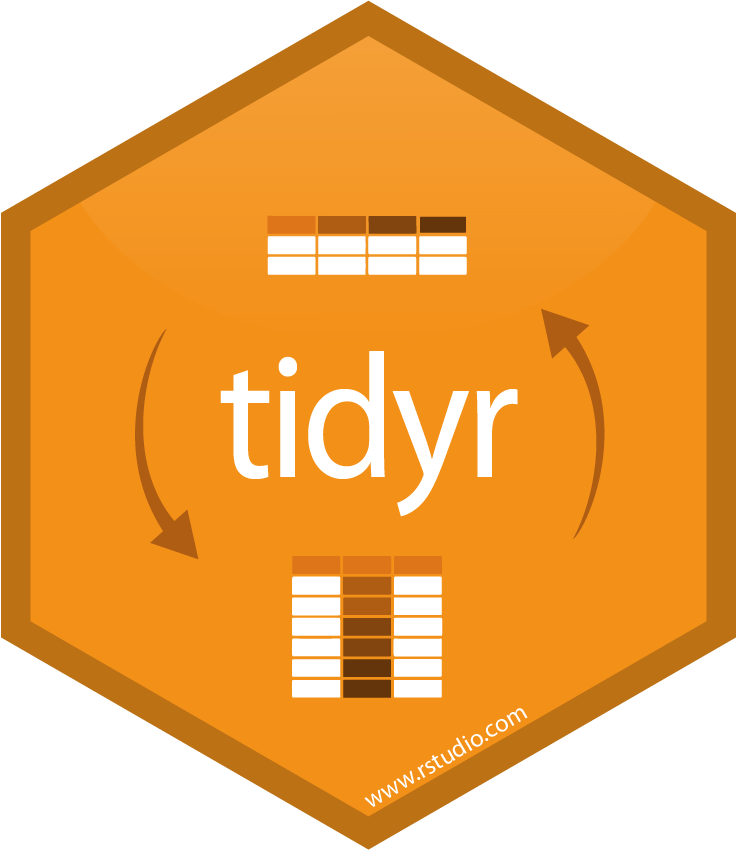
\includegraphics[width=0.25\linewidth]{imagens/tidyr} \end{center}

O pacote tidyr tem como principal objetivo transformar um data frame para o formato tidy, ou limpo.

De acordo com as regras ditas anteriormente, um dado limpo é aquele com formato \emph{long}, ou seja, com mais linhas. O outro formato é chamado de \emph{wide}, com mais colunas. No caso deste exemplo, ano é uma variável, logo é necessário existir uma coluna com os valores de ano. O valor relacionado a UF naqueles anos também é outra variável, então precisa de uma coluna pra representá-lo. Além disso, a própria UF precisa de uma coluna.

O \texttt{tidyr} possui duas funções principais:

\texttt{gather}: Transforma um \texttt{tibble} \emph{wide} em \emph{long}, ou seja, transforma os dados no formato \emph{tidy}.

\texttt{spread}: Transforma um \texttt{tibble} \emph{long} em \emph{wide}, ou seja, transforma dados que estão no formato \emph{tidy} em formato não \emph{tidy}.

Além disso, existem duas funções que podem ser importantes na nossa análise: \texttt{separate} e \texttt{unite}, que separa uma coluna em duas e vice versa.

\hypertarget{gather}{%
\subsection{\texorpdfstring{\texttt{gather}}{gather}}\label{gather}}

Vamos criar um \texttt{tibble} no formato \emph{wide} e transformá-lo em um dado \emph{tidy}:

\begin{Shaded}
\begin{Highlighting}[]
\KeywordTok{library}\NormalTok{(tibble)}
\NormalTok{tb <-}\StringTok{ }\KeywordTok{tibble}\NormalTok{(}\DataTypeTok{uf =} \KeywordTok{c}\NormalTok{(}\StringTok{"RJ"}\NormalTok{, }\StringTok{"SP"}\NormalTok{), }\StringTok{`}\DataTypeTok{2017}\StringTok{`}\NormalTok{ =}\StringTok{ }\KeywordTok{c}\NormalTok{(}\DecValTok{10}\NormalTok{, }\DecValTok{11}\NormalTok{), }\StringTok{`}\DataTypeTok{2018}\StringTok{`}\NormalTok{ =}\StringTok{ }\KeywordTok{c}\NormalTok{(}\DecValTok{11}\NormalTok{, }\DecValTok{10}\NormalTok{))}
\NormalTok{tb}
\end{Highlighting}
\end{Shaded}

\begin{verbatim}
## # A tibble: 2 x 3
##   uf    `2017` `2018`
##   <chr>  <dbl>  <dbl>
## 1 RJ        10     11
## 2 SP        11     10
\end{verbatim}

\hypertarget{transformauxe7uxe3o-de-dados-com-dplyr}{%
\chapter{\texorpdfstring{Transformação de Dados com \texttt{dplyr}}{Transformação de Dados com dplyr}}\label{transformauxe7uxe3o-de-dados-com-dplyr}}

\hypertarget{introduuxe7uxe3o}{%
\section{Introdução}\label{introduuxe7uxe3o}}

A visualização é uma ferramenta importante para a geração de \emph{insights}, mas é raro você obter os dados exatamente da forma correta de que precisa. Freqüentemente, você precisará criar algumas novas variáveis ou resumos, ou talvez apenas queira renomear as variáveis ou reordenar as observações para tornar os dados um pouco mais fáceis de trabalhar. Você aprenderá como fazer tudo isso (e muito mais!) Neste capítulo, que ensinará como transformar seus dados usando o pacote \texttt{dplyr} e um novo conjunto de dados em voos partindo de Nova York em 2013.

\hypertarget{pruxe9-requisitos-1}{%
\section{Pré-requisitos}\label{pruxe9-requisitos-1}}

Neste capítulo, vamos nos concentrar em como usar o pacote \texttt{dplyr}, outro membro central do \texttt{tidyverse}. Ilustraremos as ideias principais usando dados do pacote \texttt{nycflights13} e usaremos o \texttt{ggplot2} para nos ajudar a entender os dados.

\begin{Shaded}
\begin{Highlighting}[]
\KeywordTok{library}\NormalTok{(nycflights13)}
\KeywordTok{library}\NormalTok{(tidyverse) }\CommentTok{# ou isoladamente: library(dplyr).}
\end{Highlighting}
\end{Shaded}

\hypertarget{nycflights13}{%
\section{nycflights13}\label{nycflights13}}

Esse data frames contém todos os 336.776 vôos que partiram de Nova York em 2013. Os dados são do \href{https://www.transtats.bts.gov/DatabaseInfo.asp?DB_ID=120\&Link=0}{Bureau of Transportation Statistics} dos EUA e estão documentados em \texttt{?flights}.

\begin{Shaded}
\begin{Highlighting}[]
\NormalTok{flights}
\end{Highlighting}
\end{Shaded}

\begin{verbatim}
## # A tibble: 336,776 x 19
##     year month   day dep_time sched_dep_time dep_delay arr_time
##    <int> <int> <int>    <int>          <int>     <dbl>    <int>
##  1  2013     1     1      517            515         2      830
##  2  2013     1     1      533            529         4      850
##  3  2013     1     1      542            540         2      923
##  4  2013     1     1      544            545        -1     1004
##  5  2013     1     1      554            600        -6      812
##  6  2013     1     1      554            558        -4      740
##  7  2013     1     1      555            600        -5      913
##  8  2013     1     1      557            600        -3      709
##  9  2013     1     1      557            600        -3      838
## 10  2013     1     1      558            600        -2      753
## # ... with 336,766 more rows, and 12 more variables: sched_arr_time <int>,
## #   arr_delay <dbl>, carrier <chr>, flight <int>, tailnum <chr>,
## #   origin <chr>, dest <chr>, air_time <dbl>, distance <dbl>, hour <dbl>,
## #   minute <dbl>, time_hour <dttm>
\end{verbatim}

Para ver todo o conjunto de dados, você pode executar o \texttt{View(flights)} que abrirá o conjunto de dados no visualizador do RStudio. Imprime de forma distinta do data frame, porque é um \texttt{tibble}. O que é um \emph{tibble}?
\emph{Tibbles} são similares aos \emph{data frames}, porém diferentes em dois aspectos: \textbf{impressão} e \textbf{indexação}

Na impressão no console, os \emph{tibbles} apresentam apenas as dez primeiras linhas e todas as colunas que cabem na tela, tornando mais fácil o trabalho com grandes volumes de dados. Além disso, cada coluna apresenta o seu tipo, algo semelhante ao apresentado quando utilizamos a função \texttt{str()}. A segunda diferença, não menos importante, é a forma de indexação. Para indexar um \texttt{tibble} devemos utilizar o nome completo da variável que desejamos. Caso contrário, ocorrerá um erro.

Ainda sobre a indexação, sempre que indexarmos um \texttt{tibble} usando \texttt{{[}}, o resultado será outro \texttt{tibble}. Usando \texttt{{[}{[}} o resultados será um vetor.

Abreviações de letras sob os nomes das colunas. Eles descrevem o tipo de cada variável:

-\texttt{int} significa números inteiros;

-\texttt{dbl} significa números duplos ou reais;

-\texttt{chr} significa vetores de caracteres ou seqüências de caracteres;

-\texttt{dttm} significa data e hora (uma data + uma hora).

-\texttt{lgl} significa vetores lógicos que contêm apenas \texttt{TRUE} ou \texttt{FALSE};

-\texttt{fctr} significa fatores, que R usa para representar variáveis categóricas com valores possíveis fixos.

-\texttt{data} significa data.

Existem outros tipos comuns de variáveis que não são usadas neste conjunto de dados.

Em síntese, \emph{data frames} são tabelas de dados. Em seu formato, são bem parecidos com as matrizes, no entanto, possuem algumas diferenças significativas. Podemos idealizar os \emph{data frames} como sendo matrizes em que cada coluna pode armazenar um tipo de dado diferente. Logo, estamos lidando com um objeto bem mais versátil do que as matrizes e os vetores.

Uma das funções básicas mais importantes para começarmos a trabalhar com \emph{data frames} é a \texttt{str()}. Essa função dá uma visão clara da estrutura do nosso objeto, bem como informa os tipos de dados existentes.

\hypertarget{exercuxedcios}{%
\subsection{Exercícios}\label{exercuxedcios}}

\begin{itemize}
\tightlist
\item
  1.Qual a diferença entre uma matriz e um data frame no R?
\item
  2.Os data frames podem ser indexados com a mesma sintaxe utilizada para matrizes?
\item
  3.Qual função básica que utilizamos para verificar a estrutura dos dados de um data frame?
\end{itemize}

\hypertarget{operador-pipe}{%
\section{\texorpdfstring{Operador \emph{pipe} \texttt{\%\textgreater{}\%}}{Operador pipe \%\textgreater\%}}\label{operador-pipe}}

\begin{center}
\includegraphics[width=0.25\linewidth]{imagens/magritt} \end{center}

Os tubos são uma ferramenta poderosa para expressar claramente uma sequência de várias operações. O pipe, \texttt{\%\textgreater{}\%} vem do pacote \texttt{magrittr} de Stefan Milton Bache. Pacotes no \texttt{tidyverse} carregam \texttt{\%\textgreater{}\%} automaticamente, para que normalmente não carregue o magrittr explicitamente.

Para começar a utilizar o \emph{pipe}, instale e carregue o pacote \texttt{magrittr}.

\begin{Shaded}
\begin{Highlighting}[]
\KeywordTok{install.packages}\NormalTok{(}\StringTok{"magrittr"}\NormalTok{)}
\KeywordTok{library}\NormalTok{(magrittr)}
\end{Highlighting}
\end{Shaded}

Para mais informações sobre o \emph{pipe}, outros operadores relacionados e exemplos de utilização, visite a página \href{https://cran.r-project.org/web/packages/magrittr/vignettes/magrittr.html}{Ceci n'est pas un pipe}

\hypertarget{exercuxedcios-1}{%
\subsection{Exercícios}\label{exercuxedcios-1}}

\begin{itemize}
\item
  \begin{enumerate}
  \def\labelenumi{\arabic{enumi}.}
  \tightlist
  \item
    Reescreva a expressão abaixo utilizando o \texttt{\%\textgreater{}\%}.
  \end{enumerate}
\end{itemize}

\begin{quote}
round(mean(sum(1:10)/3), digits = 1)
\end{quote}

\textbf{Dica}: utilize a função \texttt{magrittr::divide\_by()}. Veja o help da função para mais informações.

\begin{itemize}
\item
  \begin{enumerate}
  \def\labelenumi{\arabic{enumi}.}
  \setcounter{enumi}{1}
  \tightlist
  \item
    Reescreva o código abaixo utilizando o \texttt{\%\textgreater{}\%}.
  \end{enumerate}
\end{itemize}

\begin{quote}
x \textless- rnorm(100)
x.pos \textless- x{[}x\textgreater0{]}
media \textless- mean(x.pos)
saida \textless- round(media, 1)
\end{quote}

\begin{itemize}
\item
  \begin{enumerate}
  \def\labelenumi{\arabic{enumi}.}
  \setcounter{enumi}{2}
  \tightlist
  \item
    Sem rodar, diga qual a saída do código abaixo. Consulte o \texttt{help} das funções caso precise.
  \end{enumerate}
\end{itemize}

\begin{quote}
2 \%\textgreater\%
add(2) \%\textgreater\%
c(6, NA) \%\textgreater\%
mean(na.rm = T) \%\textgreater\%
equals(5)
\end{quote}

\hypertarget{filter}{%
\section{\texorpdfstring{\texttt{filter()}}{filter()}}\label{filter}}

\texttt{filter()} permite agrupar observações com base em seus valores. O primeiro argumento da função é o nome do data frames. Por exemplo, podemos selecionar todos os valores

\hypertarget{comparauxe7uxf5es}{%
\subsection{Comparações}\label{comparauxe7uxf5es}}

\hypertarget{operadores-luxf3gicos}{%
\subsection{Operadores Lógicos}\label{operadores-luxf3gicos}}

\hypertarget{valores-ausentes}{%
\subsection{Valores Ausentes}\label{valores-ausentes}}

\hypertarget{exercuxedcios-2}{%
\subsection{Exercícios}\label{exercuxedcios-2}}

\hypertarget{arrange}{%
\section{\texorpdfstring{\texttt{arrange()}}{arrange()}}\label{arrange}}

\hypertarget{exercuxedcios-3}{%
\subsection{Exercícios}\label{exercuxedcios-3}}

\hypertarget{select}{%
\section{\texorpdfstring{\texttt{select()}}{select()}}\label{select}}

\hypertarget{exercuxedcios-4}{%
\subsection{Exercícios}\label{exercuxedcios-4}}

\hypertarget{mutate}{%
\section{\texorpdfstring{\texttt{mutate()}}{mutate()}}\label{mutate}}

\hypertarget{funuxe7uxf5es-uxfateis-de-criauxe7uxe3o}{%
\subsection{Funções úteis de criação}\label{funuxe7uxf5es-uxfateis-de-criauxe7uxe3o}}

\hypertarget{exercuxedcios-5}{%
\subsection{Exercícios}\label{exercuxedcios-5}}

\hypertarget{summarise}{%
\section{\texorpdfstring{\texttt{summarise()}}{summarise()}}\label{summarise}}

\hypertarget{combinando-vuxe1rias-operauxe7uxf5es-com-pipe}{%
\subsection{\texorpdfstring{\texttt{\%\textgreater{}\%} Combinando várias operações com pipe}{\%\textgreater\% Combinando várias operações com pipe}}\label{combinando-vuxe1rias-operauxe7uxf5es-com-pipe}}

\hypertarget{group_by}{%
\section{\texorpdfstring{\texttt{group\_by()}}{group\_by()}}\label{group_by}}

\hypertarget{manipulando-data-frames-com-dplyr}{%
\chapter{\texorpdfstring{Manipulando Data Frames com \texttt{dplyr}}{Manipulando Data Frames com dplyr}}\label{manipulando-data-frames-com-dplyr}}

\hypertarget{data-frames}{%
\section{Data Frames}\label{data-frames}}

\hypertarget{final-words}{%
\chapter{Final Words}\label{final-words}}

We have finished a nice book.

\bibliography{book.bib,packages.bib}


\end{document}
